% source https://docs.google.com/presentation/d/1j9GgVLT7fVKHwGSrdbd9HCPcR_T5TcIIF5dhADAEKsk
\begin{figure}
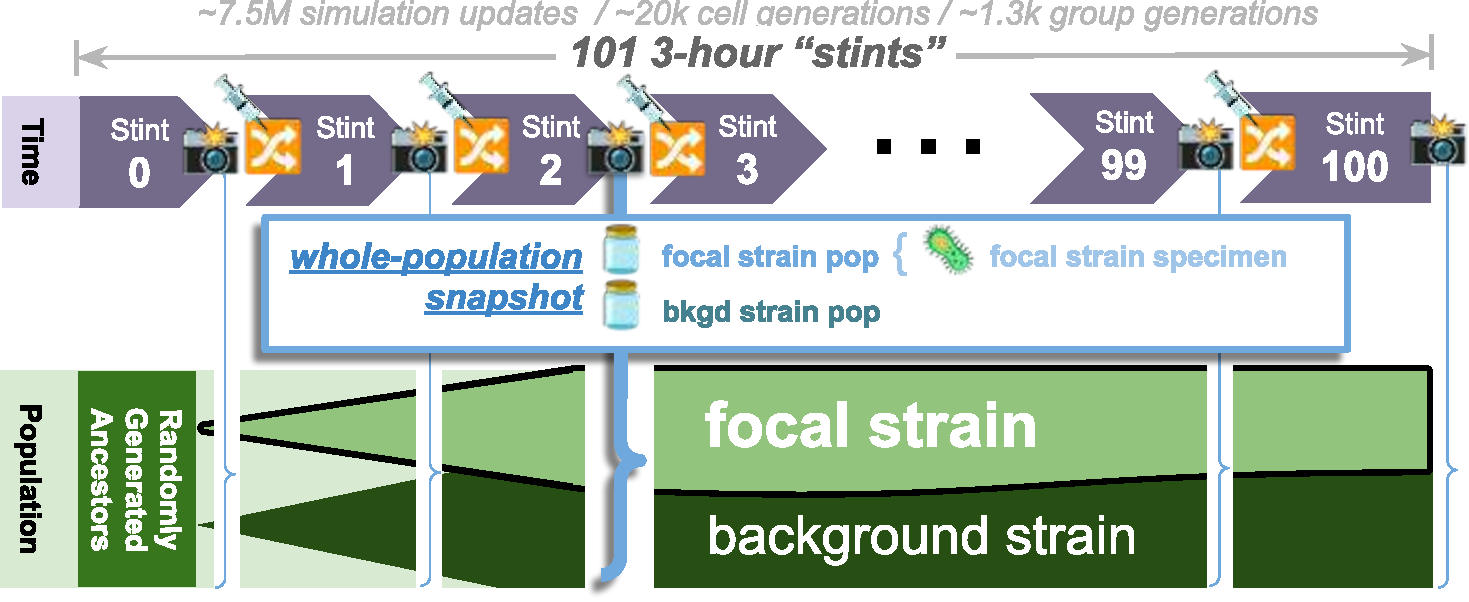
\includegraphics[width=\linewidth]{{img/stints.pdf}}
\caption{%
\textbf{Evolutionary regimen.}
\footnotesize
Experiment was initialized with founder population of randomly-generated.
Among founder lineages, an arbitrary clade was designated as ``focal strain'' subject of case study.
To ensure genomes maintained viability as simulation seeds (e.g., for competition and monoculture trials) and provide checkpoints in the case of cluster downtime, population was subjected to serial passage between 3-hour simulation windows --- referred to as ``stints.''
Between stints, a whole-population snapshot of genome content was recorded --- allowing later isolation of focal and background strain subpopulations, as well as a sample focal strain genome (``focal specimen'').
To continue evolution in the following stint, a fresh simulation instance was initialized via a shuffled injection of snapshot genomes.
Note that, due to early extinctions, an initially-secondary strain gained focal designation at stint 2, which was maintained onwards.
A diversity-maintenance procedure was used to ensure stable long-term coexistence between at least two founder lineages, hence ensuring preservation of an independent ``background'' strain.
}
\label{fig:stints}
\end{figure}
